%% -*- coding: utf-8; -*-

\documentclass[
  msc
]{ThesisPUC}


%%%
%%% Additional Packages
%%%

  %% \usepackage[brazilian]{babel}      %% in ThesisPUC.cls
  %% \usepackage[utf8]{inputenc}        %% .
  %% \usepackage[T1]{fontenc}           %% .
  %% \usepackage{lmodern}               %% .
  %% \usepackage[pdftex]{graphicx}	%% .

  \usepackage{tabularx}
  \usepackage{multirow}
  \usepackage{multicol}
  \usepackage{colortbl}
  \usepackage[%
    dvipsnames,
    svgnames,
    x11names,
    fixpdftex
  ]{xcolor}
  \usepackage{numprint}
  \usepackage{textcomp}
  \usepackage{booktabs}
  \usepackage{amsmath}
  \usepackage{enumitem}
  \usepackage{amssymb}
  \usepackage{textcomp}
  
  \usepackage{float}
  \usepackage{color,colortbl,array}
  \definecolor{GrayJ}{gray}{0.85}
  
  \usepackage{cite}
  \renewcommand\citeleft{[}
  \renewcommand\citeright{]}
  
  \graphicspath{{images/}}


%% numprint 
\npthousandsep{.}
\npdecimalsign{,}

%% ThesisPUC option
%\tablesmode{figtab} %% [nada, fig, tab ou figtab]

\setcounter{tocdepth}{3}
\setcounter{secnumdepth}{3}


%%%
%%% New commands and other global definitions
%%%

% -*- coding: iso-8859-1; -*-

%%%
%%% Newcommands
%%%

\newcommand{\degree}{\ensuremath{^\circ}}

\newcommand{\cetem}{Centro de Tecnologia Mineral}

\newcommand{\mybulletOB}{%
  % \textbullet
  % \checkmark
  $\triangleright$
  %\textopenbullet
}

\newcolumntype{L}{>{\raggedright \arraybackslash}X}
\newcolumntype{R}{>{\raggedleft \arraybackslash}X}
\newcolumntype{C}{>{\centering \arraybackslash}X}
\newcolumntype{M}[1]{>{\centering\hspace{0pt}}m{#1}}

\newcommand{\mrcel}[2]{%
\begin{tabular}[c]{@{}c@{}}#1\\#2\end{tabular}}

\newcommand{\mrcell}[2]{%
\begin{tabular}[l]{@{}l@{}}#1\\#2\end{tabular}}

\newcommand{\mrcelthree}[3]{%
\begin{tabular}[c]{@{}c@{}c@{}}#1\\#2\\#3\end{tabular}}

\newcommand{\mrcelcolorg}[2]{%
\begin{tabular}{l}\rowcolor{Gainsboro}#1\\#2\end{tabular}}

\newcommand{\mytbcimg}[3]{%
  \multicolumn{1}{C}{\parbox[c]{#1}{\includegraphics[width=#2]{#3}}}}



%%%
%%% Titulos
%%%

\author{Jorge Salvador Paredes Merino}
\authorR{Paredes Merino, Jorge Salvador}

\adviser{Ricardo Tanscheit}{Prof.}
\adviserR{Tanscheit, Ricardo}

\coadviser{Marley Maria Bernardes Rebuzzi Vellasco}{Dr.}
\coadviserR{Vellasco, Marley Maria Bernardes Rebuzzi}
%\coadviserInst{Centro de Tecnologia Mineral}{CETEM/MCTI}

\title{Síntese Automática de Sistemas de Inferência Fuzzy para Classificação}

\titleuk{Automatic Synthesis of Fuzzy Inference Systems for Classification}

%% \subtitulo{Aqui vai o subtitulo caso precise}

\day{21}
\month{Dezembro}
\year{2015}

\city{Rio de Janeiro}
\CDD{620.11}
\department{Engenharia Elétrica}
\program{Processamento de Sinais e Controle}
\school{Centro Técnico Científico}
\university{Pontifícia Universidade Católica do Rio de Janeiro}
\uni{PUC-Rio}


%%%
%%% Jury
%%%

\jury{%
	\jurymember{Jorge Luís Machado do Amaral}{Prof.}
	{Faculdade de Engenharia}{UERJ}
	\jurymember{Karla Tereza Figueiredo Leite}{Prof.}
	{Departamento de Engenharia Elétrica}{PUC-Rio}
  \schoolhead{José Eugenio Leal}{Prof.}
}


%%%
%%% Resume
%%%

\resume{%
Graduou-se em Engenharia Mecatrónica pela Universidad Nacional de Ingeniería (Lima, Perú)...}


%%%
%%% Acknowledgment
%%%

\acknowledgment{%
  Em primeiro lugar, gostaria de agradecer especialmente a ...
}


%%%
%%% Keywords
%%%

\keywords{%
	\key{Sistemas de Inferência Fuzzy;}
	\key{Classificação;}
	\key{Interpretabilidade;}
}

\keywordsuk{%
	\key{Fuzzy Inference System;}%
	\key{Classification;}%
	\key{Interpretability;}%
}


%%%
%%% Abstract
%%%

\abstract{%
  Hoje em dia, grande parte do ...
}

\abstractuk{%
  Nowadays, much of the ...}


%%%
%%% Epigraph
%%%

\epigraph{%
	Cada livro, cada volume que vês, tem alma. A alma de quem o escreveu e a alma dos que o leram e viveram e sonharam com ele. Cada vez que um livro muda de mãos, cada vez que alguém desliza o olhar pelas suas páginas, o seu espírito cresce e torna-se forte.
}
\epigraphauthor{Carlos Ruiz Zafón}
\epigraphbook{A sombra do vento}


%%%
%%% 
%%%

\begin{document}

  %% -*- coding: utf-8; -*-

\begin{thenotations}

  \noindent
  \begin{tabular}{ll}
    SFI -- Sistemas de Inferência Fuzzy\\
    SFE -- Sistemas Fuzzy Evoluacionários\\
    BC -- Base de Conhecimento\\
    BP -- Base de Parâmetros\\
  \end{tabular}

\end{thenotations}

  % -*- coding: utf-8; -*-

\chapter{Introdução}

...

Definem-se\cite{Gacto2011} os Quadrantes de Interpretabilidade apresentados na Figura \ref{fig:1-1} ...

\begin{figure} [h]
  \begin{center}
    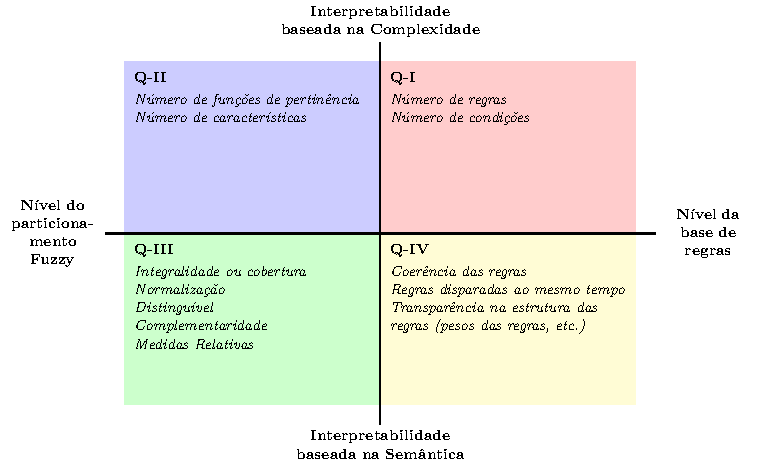
\includegraphics[width=11cm]{cap1/quadrantesInterpretability.ps}
    \caption{Indicadores nos Quadrantes de Interpretabilidade}\label{fig:1-1}
  \end{center}
\end{figure}

  % -*- coding: utf-8; -*-

\chapter{Estudo de casos}

Este capítulo apresenta uma série de estudos de casos resumidos na Figura \ref{fig:2-3} ...

\begin{figure} [h]
	\begin{center}
		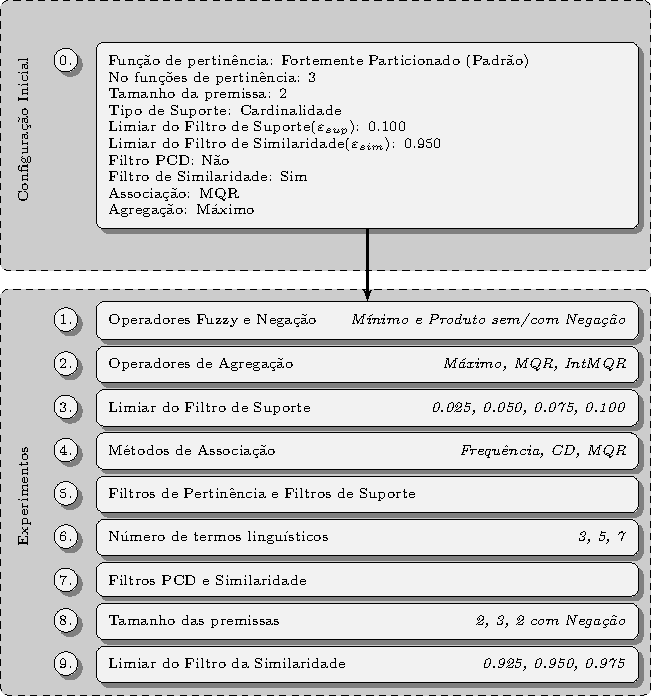
\includegraphics[width=12cm]{cap2/Experimentos.ps}
		\caption{Delineamento sequencial dos Experimentos avaliados para o modelo AutoFIS-Class}\label{fig:2-3}
	\end{center}
\end{figure}

...

Os resultados do Experimento 2 são apresentados na Tabela \ref{Exp2Ac-Nr}:

% -*- coding: utf-8; -*-

\begin{table}[H]
\begin{centering}
\begin{tabular}{rlcccccccc}
 \toprule
 \multicolumn{1}{c}{} & \multicolumn{1}{c}{} & \multicolumn{3}{c}{Acurácia} & \multicolumn{3}{c}{Número de regras}\tabularnewline
 \cmidrule(lr){3-5} \cmidrule(lr){6-8}
& Base de dados & Máximo & MQR & IntMQR & Máximo & MQR & IntMQR\\ 
 \hline
  1 & appendicitis & 65.18 & 87.09 & \textbf{87.91} & 9.70 & \cellcolor[gray]{0.85}5.30 & 6.70 \\
  2 & australian & 79.57 & 85.51 & \textbf{85.80} & 20.50 & \cellcolor[gray]{0.85}13.80 & 18.40 \\
  3 & balance & 62.10 & \textbf{89.59} & 78.59 & 57.30 & \cellcolor[gray]{0.85}23.80 & \cellcolor[gray]{0.85}23.80 \\
  4 & banana & 56.04 & \textbf{60.21} & 52.64 & 10.80 & 6.00 & \cellcolor[gray]{0.85}4.20 \\
  5 & bupa & 56.11 & \textbf{62.33} & 58.81 & 14.30 & \cellcolor[gray]{0.85}7.50 & 8.30 \\
  6 & cleveland & 56.54 & \textbf{59.27} & 58.63 & 75.00 & \cellcolor[gray]{0.85}48.40 & 52.70 \\
  7 & contraceptive & 43.59 & \textbf{52.07} & 50.58 & 49.00 & 28.70 & \cellcolor[gray]{0.85}28.40 \\
  8 & crx & 74.60 & 86.30 & \textbf{86.45} & 20.60 & \cellcolor[gray]{0.85}13.10 & 15.00 \\
  9 & ecoli & 36.34 & \textbf{72.89} & 71.12 & 76.80 & \cellcolor[gray]{0.85}46.60 & 73.50 \\
  10 & glass & 45.51 & \textbf{58.68} & 50.81 & 37.00 & \cellcolor[gray]{0.85}21.00 & 27.60 \\
  11 & haberman & 69.28 & \textbf{75.13} & 73.51 & 16.30 & 9.10 & \cellcolor[gray]{0.85}8.70 \\
  12 & hayes-roth & 45.00 & \textbf{64.38} & 56.25 & 33.50 & \cellcolor[gray]{0.85}17.90 & 78.20 \\
  13 & heart & 68.15 & \textbf{86.30} & 84.81 & 21.10 & \cellcolor[gray]{0.85}13.10 & 17.20 \\
  14 & hepatitis & 83.43 & \textbf{85.23} & 83.65 & 26.00 & 15.50 & \cellcolor[gray]{0.85}14.80 \\
  15 & iris & 76.67 & 95.33 & \textbf{96.67} & 11.90 & \cellcolor[gray]{0.85}6.00 & 6.80 \\
  16 & magic & 65.04 & \textbf{77.38} & 76.37 & 12.70 & 6.50 & \cellcolor[gray]{0.85}5.90 \\
  17 & monk-2 & 52.66 & 91.10 & \textbf{94.09} & 30.10 & 9.70 & \cellcolor[gray]{0.85}6.80 \\
  18 & newthyroid & 77.29 & \textbf{84.74} & 83.79 & 12.50 & \cellcolor[gray]{0.85}8.40 & 10.10 \\
  19 & page-blocks & 86.90 & \textbf{89.80} & \textbf{89.80} & 28.40 & \cellcolor[gray]{0.85}15.70 & 16.30 \\
  20 & phoneme & 59.36 & 70.54 & \textbf{70.67} & 14.80 & \cellcolor[gray]{0.85}7.90 & 8.10 \\
  21 & pima & 56.51 & \textbf{75.27} & 73.97 & 15.10 & \cellcolor[gray]{0.85}8.70 & 11.00 \\
  22 & saheart & 58.44 & \textbf{73.83} & 73.39 & 19.00 & \cellcolor[gray]{0.85}9.60 & 12.20 \\
  23 & tae & 34.42 & \textbf{47.17} & 43.12 & 32.70 & \cellcolor[gray]{0.85}17.60 & 29.30 \\
  24 & thyroid & \textbf{92.58} & 92.21 & \textbf{92.58} & 17.80 & \cellcolor[gray]{0.85}10.60 & 23.30 \\
  25 & titanic & 67.74 & 77.65 & \textbf{78.28} & 14.20 & \cellcolor[gray]{0.85}9.70 & 13.80 \\
  26 & vehicle & 42.91 & 56.16 & \textbf{58.15} & 30.50 & \cellcolor[gray]{0.85}18.00 & 19.60 \\
  27 & vowel & 21.72 & \textbf{45.66} & 45.45 & 130.50 & 69.80 & \cellcolor[gray]{0.85}65.70 \\
  28 & wine & 72.06 & \textbf{91.47} & 86.93 & 17.60 & \cellcolor[gray]{0.85}9.60 & 10.80 \\
  29 & winequality-red & 48.09 & \textbf{57.85} & 57.66 & 46.90 & \cellcolor[gray]{0.85}27.20 & 33.60 \\
  30 & wisconsin & 90.78 & 94.45 & \textbf{96.08} & 20.60 & 13.70 & \cellcolor[gray]{0.85}12.50 \\
  31 & yeast & 39.35 & \textbf{51.62} & 51.01 & 54.90 & \cellcolor[gray]{0.85}27.60 & 37.10 \\
   \bottomrule
\end{tabular}
\par\end{centering}


\protect\caption{Acurácias das bases de dados no Experimento 2.}
\label{Exp2Ac-Nr}
\end{table}

\newpage

\section{Investigação
	Empírica da Arquitetura do Modelo AutoFIS-Class \label{sec:EmpiricResearch}}

...

\section{Extensão do modelo AutoFIS-Class}
	
Conforme indicado na Seção \ref{sec:EmpiricResearch} ...

  \arial
  \bibliography{referencias}
  \normalfont
  % -*- coding: utf-8; -*-

\appendix
\chapter{Artigo da Tese Publicado em Congresso}

O método de Sintetização Automática de Sistemas de Inferência Fuzzy para Classificação mostrado neste trabalho rendeu uma publicação no Congresso Brasileiro de Inteligência Computacional (CBIC-2015) e foi aceito para o evento do IPMU-2016 ...



\end{document}
